%----------------------------------------------------------------------------------------
%    PACKAGES AND THEMES
%----------------------------------------------------------------------------------------

\documentclass[aspectratio=169,xcolor=dvipsnames]{beamer}
\usetheme{SimpleDarkBlue}

\usepackage{hyperref}
\usepackage{graphicx} % Allows including images
\usepackage{booktabs} % Allows the use of \toprule, \midrule and \bottomrule in tables
\usepackage[absolute,overlay]{textpos}

% \usepackage[style=numeric-comp,backend=biber]{biblatex}
% \addbibresource{reference.bib}

\newcommand\myheading[1]{%
  \par\bigskip
  {\Large\bfseries#1}\par\smallskip}

% anything surronded by this new command will not do anything
\newcommand{\mycomment}[1]{}
\setbeamertemplate{bibliography item}{[\arabic{enumiv}]}
%----------------------------------------------------------------------------------------
%    TITLE PAGE
%----------------------------------------------------------------------------------------

\title{Real-Time Hyperspectral Signal Processing and Classification}
\subtitle{2025 Midterm Presentation}

\author{Nash Rickert}

\institute
{
    Electrical and Computer Engineering Department, REU \\
    Montana State University % Your institution for the title page
}
\date{\today} % Date, can be changed to a custom date

%----------------------------------------------------------------------------------------
%    PRESENTATION SLIDES
%----------------------------------------------------------------------------------------

% TODO: Add some image/presentation citations. Practice presentation and write any notes I feel are important to structure the flow of the presentation
\begin{document}

\begin{frame}
    % Print the title page as the first slide
    \titlepage
\end{frame}

% \begin{frame}{Overview}
%     % Throughout your presentation, if you choose to use \section{} and \subsection{} commands, these will automatically be printed on this slide as an overview of your presentation
%     \tableofcontents
% \end{frame}

%------------------------------------------------
% \section{First Section}
%------------------------------------------------
\begin{frame}{Introduction}
    \myheading{Overview}
    \begin{itemize}
        \item Our goal is to implement real-time hyperspectral classification. This means that our model would be integrated with the data-collection process so that there is no need to handle large amounts of data after collection.
        \begin{itemize}
            \item Currently it is often the case that large amounts of hyperspectral data will be collected in the field, then need to be processed seperately before any results can be acted upon.
        \end{itemize}
        \item This naturally means that the main goal of our project is to minimize the latency of the classification process so it matches the pace of data collection.
    \end{itemize}

    % Contrast this goal with what typically happens
    \begin{block}{Motivation}
        Real-time classification would provide immediate insight to field workers, allowing them to make important decisions quickly.
    \end{block}
\end{frame}

\begin{frame}{Background: Hyperspectral Imaging (HSI)}
    \begin{columns}
        \begin{column}{0.48\textwidth}
            \begin{itemize}
                \item HSI uses diffraction to sample a continuous range of spectral bands.
                \item Because of its high dimensionality, hyperspectral data tends to be large and difficult to process.
                \begin{itemize}
                    \item A typical RGB image has 3 channels. Our sensor uses 1604. 535x larger.
                \end{itemize}
            \end{itemize}
            \begin{figure}
                \centering
                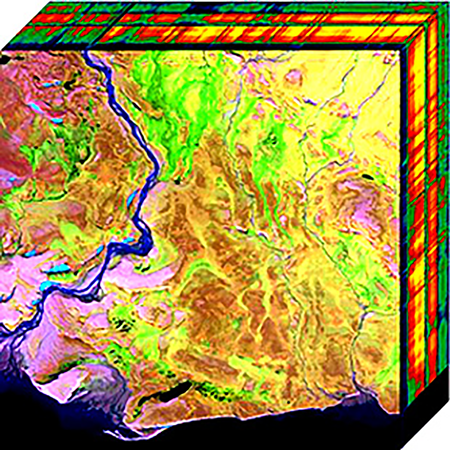
\includegraphics[width=0.5\textwidth]{datacube.png}
            \end{figure}
        \end{column}
        \begin{column}{0.48\textwidth}
            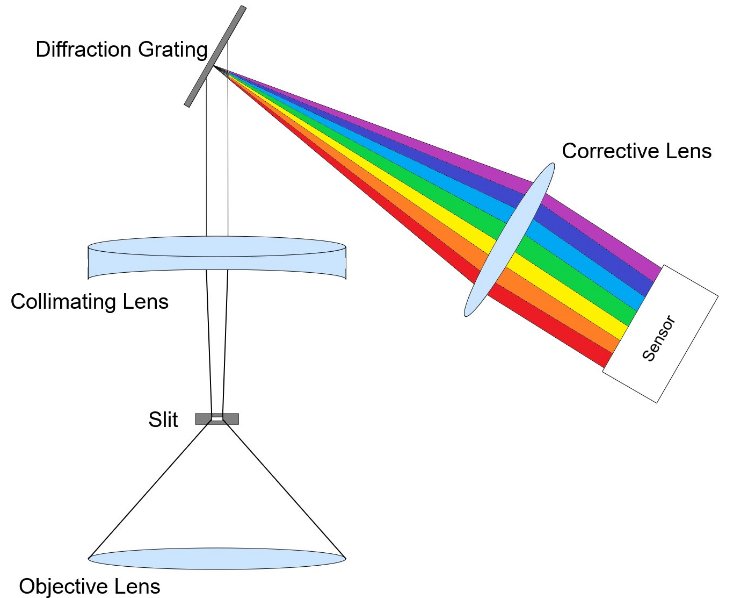
\includegraphics[width=\textwidth]{hsi_optics.png}

            \begin{textblock*}{5cm}(0.2cm,8.5cm)
                \tiny Left image: \cite{hsi-cube} \\ Right image: \cite{nat-presentation}
            \end{textblock*}
            
            % \vfill
            % {\tiny \hfill Left image: \cite{hsi-cube} \\ \hfill Right image: \cite{nat-presentation}  \par}
        \end{column}
    \end{columns}
\end{frame}

% Note: On this slide mostly want to talk about the images, point out the spectrum and the fact that we get the full spectrum for just one pixel (hence the arrows). The words are not that important
\begin{frame}{Background: HSI for Classification}
    \begin{columns}
        \begin{column}{0.53\textwidth}
            \begin{itemize}
                \item Hyperspectral imaging data can be used to classify objects in images. Their high wavelength spectrum makes them especially useful for environmental monitoring, agriculture, and more.
                \item For our project, we're interested in identifying regions of forests with an adbundance of bio-fuel which puts them at risk of forest-fires.
            \end{itemize}


            \begin{textblock*}{5cm}(0.2cm,8.5cm)
                \tiny Top image: \cite{hsi-stones} \\ Bottom image: \cite{hsi-people}
            \end{textblock*}

            % \vfill
            % {\begin{flushleft} \tiny \hfill Top image: \cite{hsi-stones} \\ \hfill Right image: \cite{hsi-people}  \par \end{flushleft}}

        \end{column}
        \begin{column}{0.43\textwidth}
            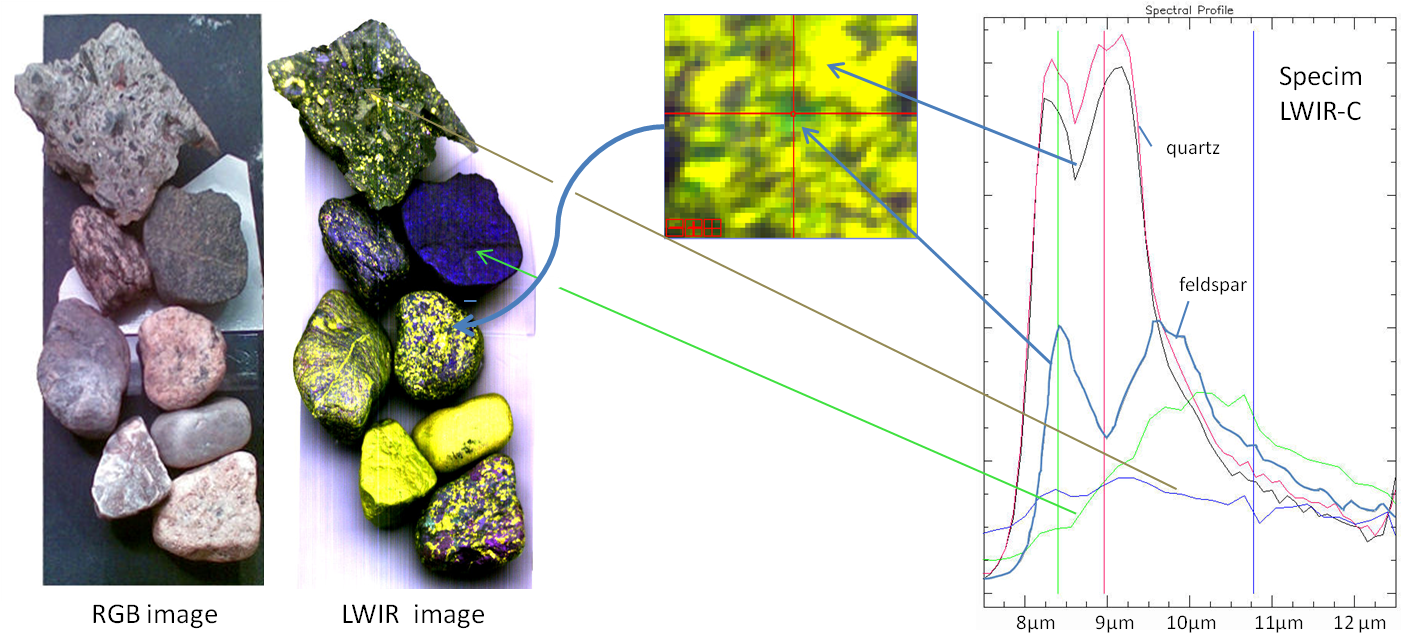
\includegraphics[width=\textwidth]{wiki_hsi2.png}
            \begin{figure}
                \centering
                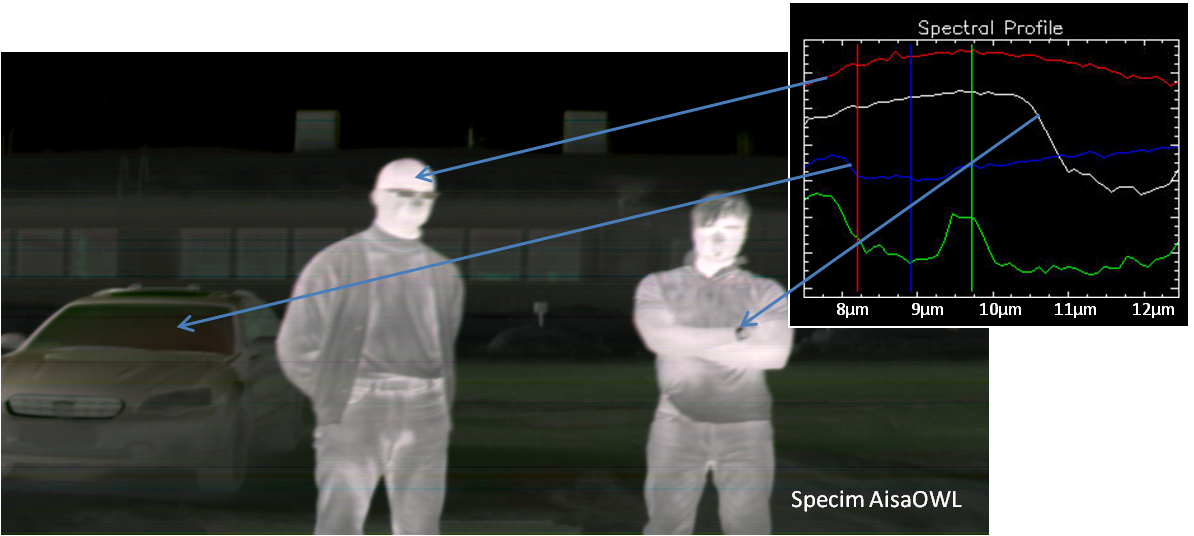
\includegraphics[width=\textwidth]{wiki_hsi1.png}
            \end{figure}
        \end{column}
    \end{columns}
\end{frame}
    

% Do mention in words the determinism vs nondeterminism of the two approaches (refresh cycles and cache misses), the potential for lower latency for FPGAs due to streaming, the fact that we get programmable i/o
\begin{frame}{Background: FPGAs}
    \begin{itemize}
        \item An FPGA (Field Programmable Gate Array) is a programmable circuit.
        \item They are built out of logic elements, DSP slices (for performing simple addition and multiplication), and local memory (consisting of static RAM).
        \item They consist of a 'fabric' of resources where everything is interconnected (hence programmable).
    \end{itemize}
    \begin{columns}
        \begin{column}{0.48\textwidth}
            \begin{figure}
                \centering
                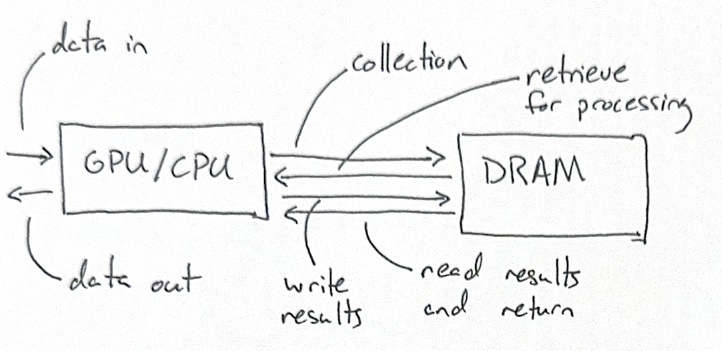
\includegraphics[width=\textwidth]{gpucpu.png}
            \end{figure}
        \end{column}
        \begin{column}{0.48\textwidth}
            \begin{figure}
                \centering
                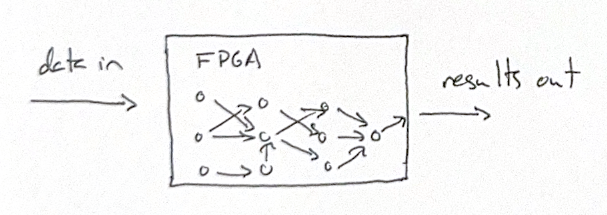
\includegraphics[width=\textwidth]{fpga.png}
            \end{figure}
        \end{column}
    \end{columns}
\end{frame}


\begin{frame}{Research Question}
    \begin{alertblock}{Research Question}
        How much can different neural network model architectures for classifying hyperspectral data improve latency in an FPGA implementation without sacrificing accuracy?
    \end{alertblock}
    \myheading{Baseline}
    \begin{itemize}
        \item Previous work at MSU successfully reduced band dimension on a HSI dataset and performed high accuracy classification on it.
        \item 99.7\% accuracy using a large convolutional neural network.
        \item Performs roughly 2 billion elementary add/multiply operations for each pixel classified.
    \end{itemize}
\end{frame}

\begin{frame}
    \begin{figure}
        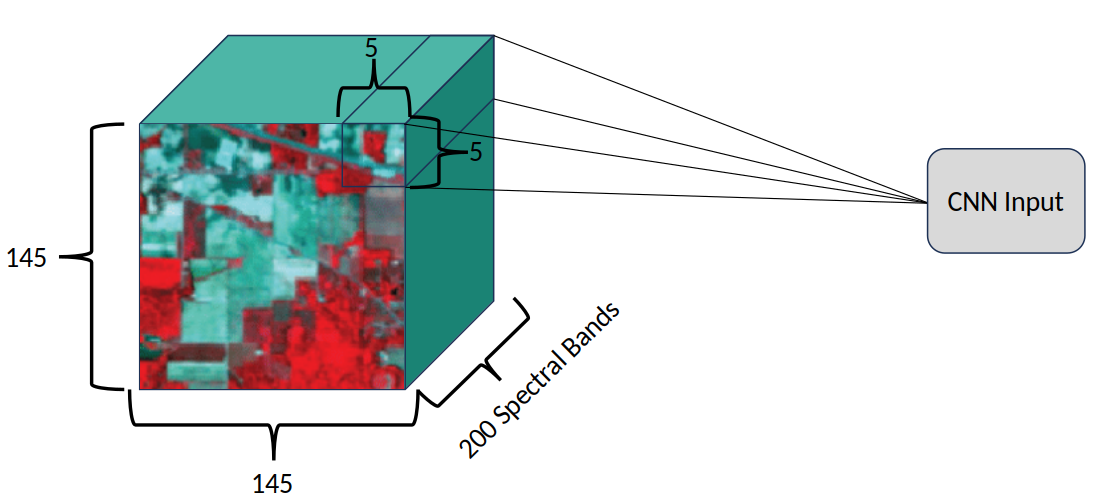
\includegraphics[width=0.5\linewidth]{cnn_data.png}
        % 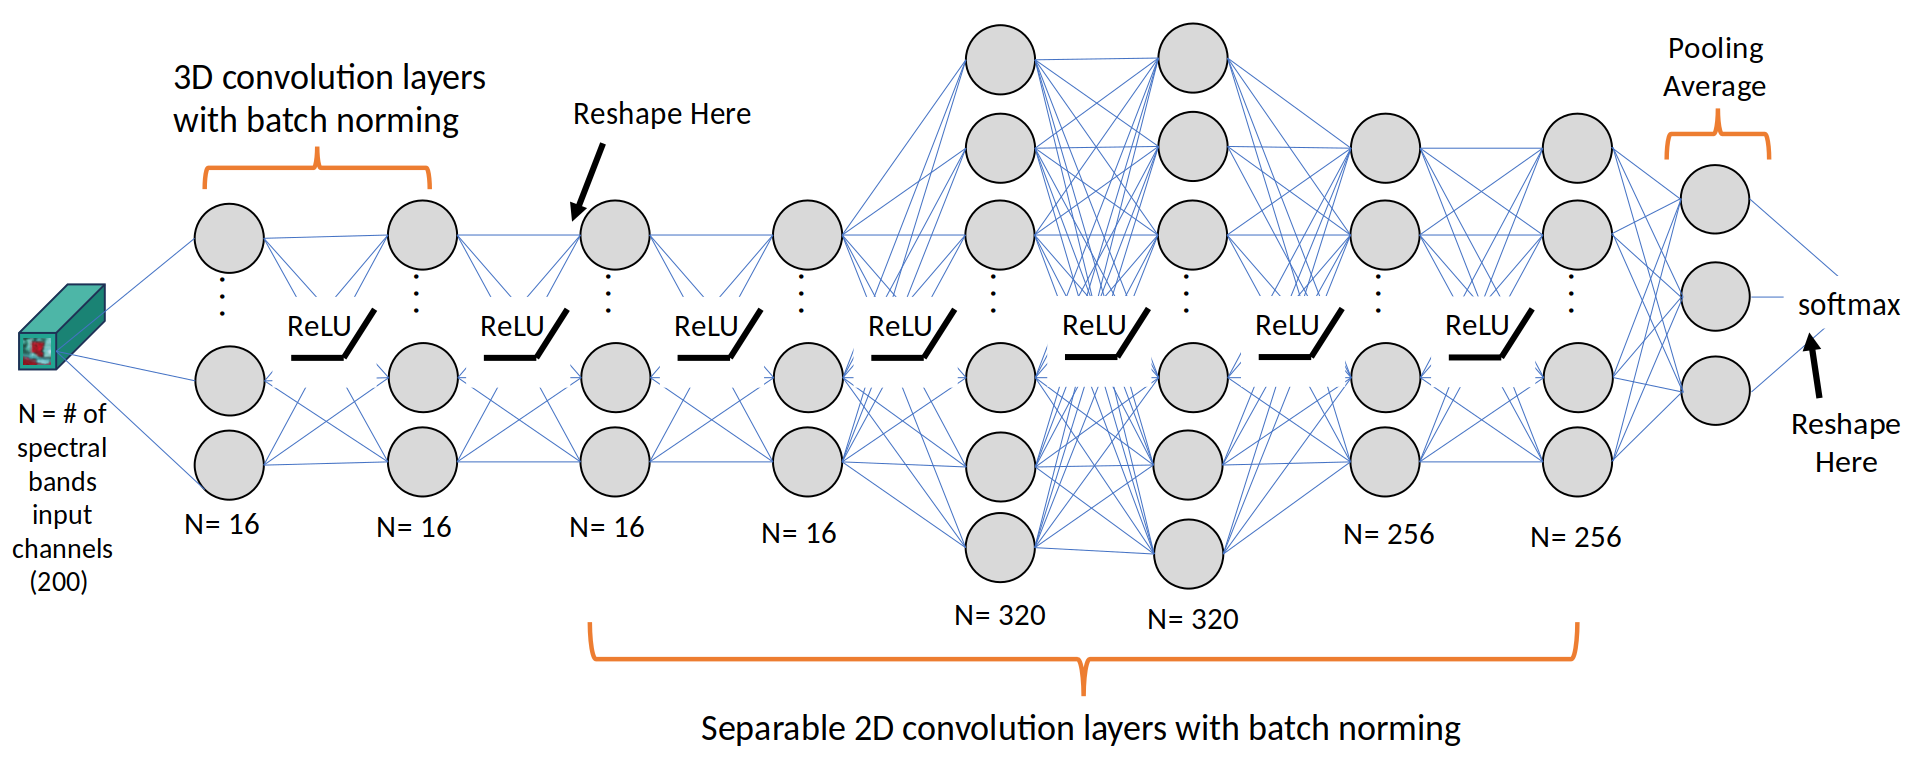
\includegraphics[width=0.7\linewidth]{cnn_arch.png}
    \end{figure}

    \begin{figure}
        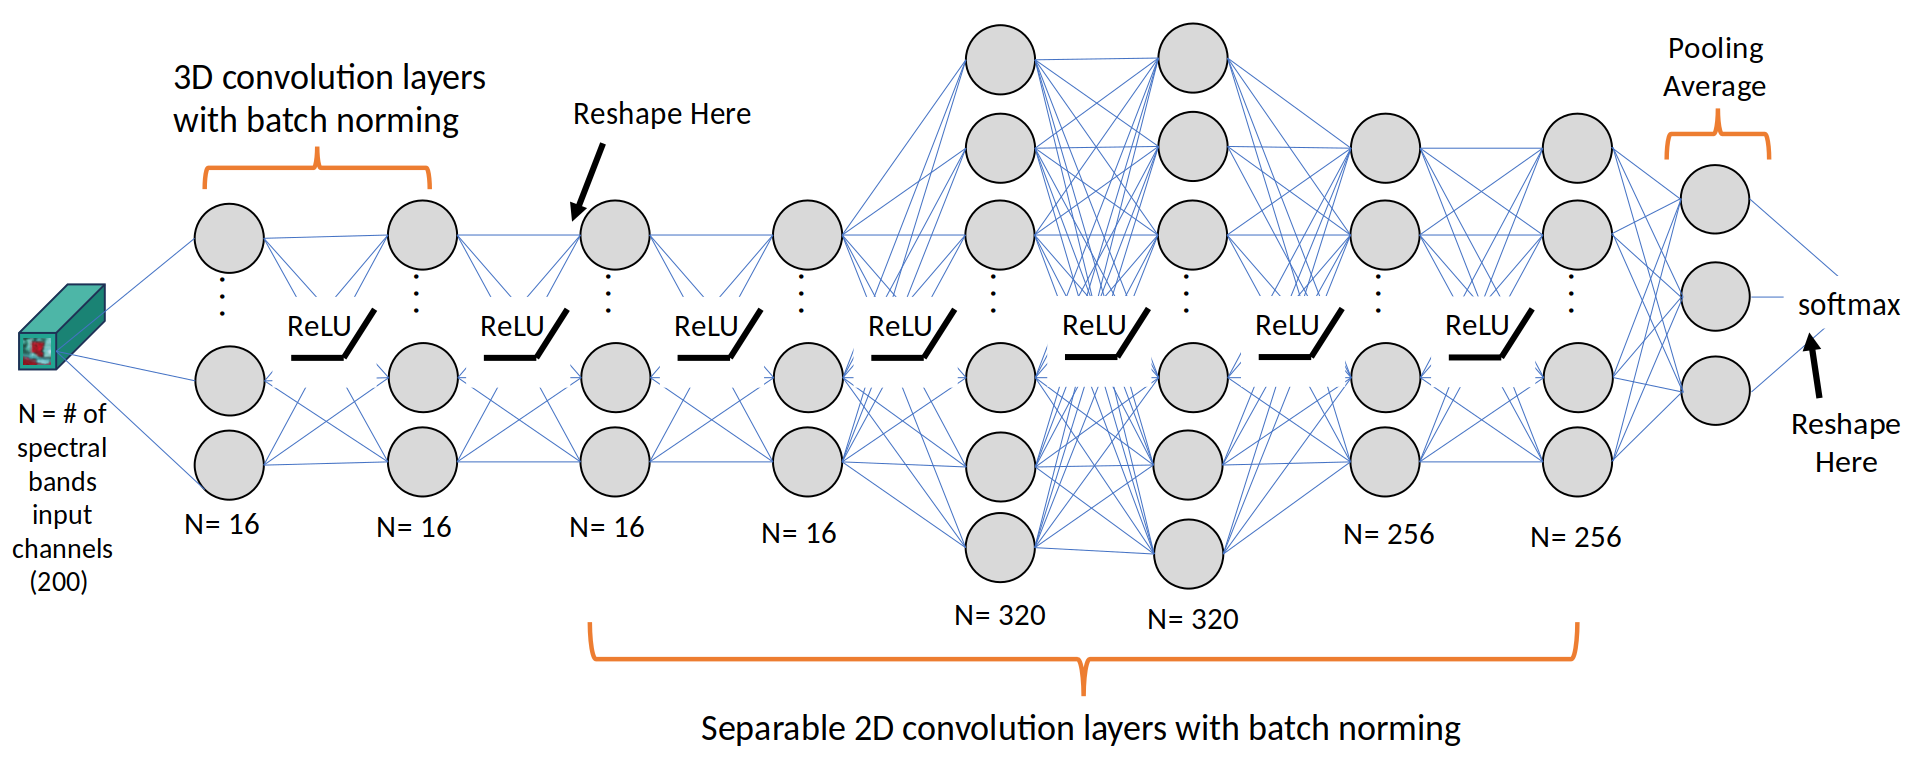
\includegraphics[width=0.8\linewidth]{cnn_arch.png} 
    \end{figure}

    \begin{textblock*}{5cm}(0.2cm,8.5cm)
        \tiny Both images: \cite{dirk-presentation}
    \end{textblock*}

\end{frame}

\begin{frame}{Alternative Architectures}
    \myheading{CNN Drawbacks}
    \begin{itemize}
        \item A CNN allows us to gain spatial information about our image by taking into account pixels around each pixel
        \begin{itemize}
            \item For real time classification, this requires storing data so our kernel can pass over it, interrupting the flow of data through our FPGA
        \end{itemize}
        \item The CNN implementations are also quite large and might not be viable for our hardware needs.
    \end{itemize}
    

    \myheading{Kolmogorov Arnold Networks (KAN)}
    % This is probably the section that I need to say the most in words. In particular, explain the differences between
    % Fixed activation + linear transformation in a traditional MLP vs learning activations directly
    \begin{itemize}
        \item Directly learns the nonlinear activation functions of a network.
        \item In an FPGA, these functions could be encoded directly as lookup tables, allowing us to approximate results much more quickly.
        \item If pixel-classification is viable, we can avoid storing/transferring data from memory for a CNN kernel. 
    \end{itemize}
\end{frame}

\begin{frame}
    \begin{figure}
        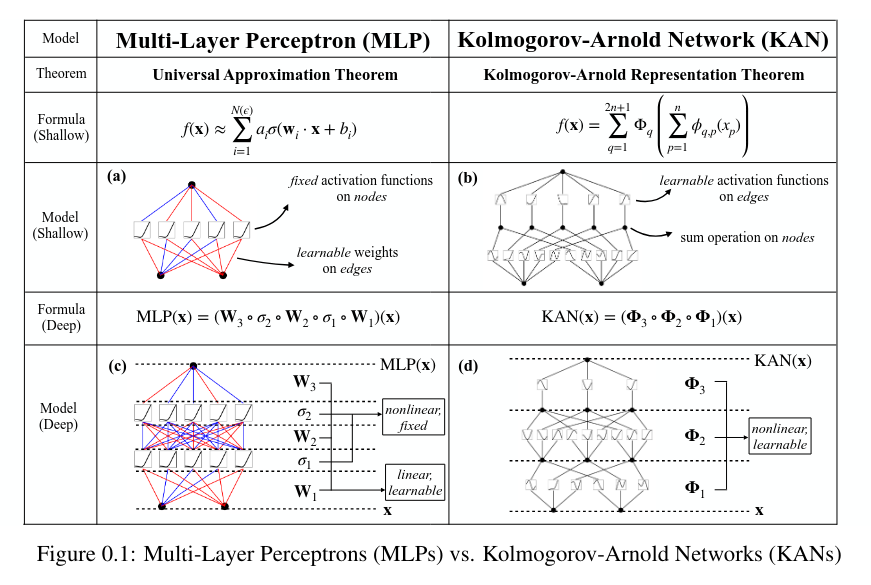
\includegraphics[width=0.75\linewidth]{mlpkan.png} 
    \end{figure}


    \begin{textblock*}{5cm}(0.2cm,8.5cm)
        \tiny Image: \cite{kan}
    \end{textblock*}

\end{frame}

\begin{frame}{Work Done}
    \begin{itemize}
        \item To properly benchmark and implement, we need to shift the models from the high level and opaque python implementations to something lower level.
        \item To do this, I transferred both the baseline CNN implementation and the KAN to C (for the latter, I created a custom C library that can be called directly from python).
        \begin{itemize}
            \item This allows us to do preliminary benchmarking and provides an interface to swap out the computational parts of the classification directly to the FPGAs.
            \item This process will likely form the basis of the rest of my work at the REU.
        \end{itemize}
        
    \end{itemize}
\end{frame}

% \begin{frame}{Project Plan}
%     \myheading{Inter-group Cooperation}
%     \begin{itemize}
%         \item Our work is a part of a broader 'SMART FIRES' initiative. Our findings on what works for our hardware can provide insight to other groups, such as the machine learning team.
%     \end{itemize}

%     \myheading{Model Distillation}
%     \begin{columns}
%         \begin{column}{0.60\textwidth}
%             \begin{itemize}
%                 \item Training data for the project is still being collected, and other teams are largely responsible for model design.
%                 \item With model distillation, we can take their results and transform it into something suitable for our hardware needs.
%             \end{itemize}

%             \begin{textblock*}{5cm}(0.2cm,8.5cm)
%                 \tiny Image: \cite{distillation}
%             \end{textblock*}

%         \end{column}
%         \begin{column}{0.40\textwidth}
%             \centering
%             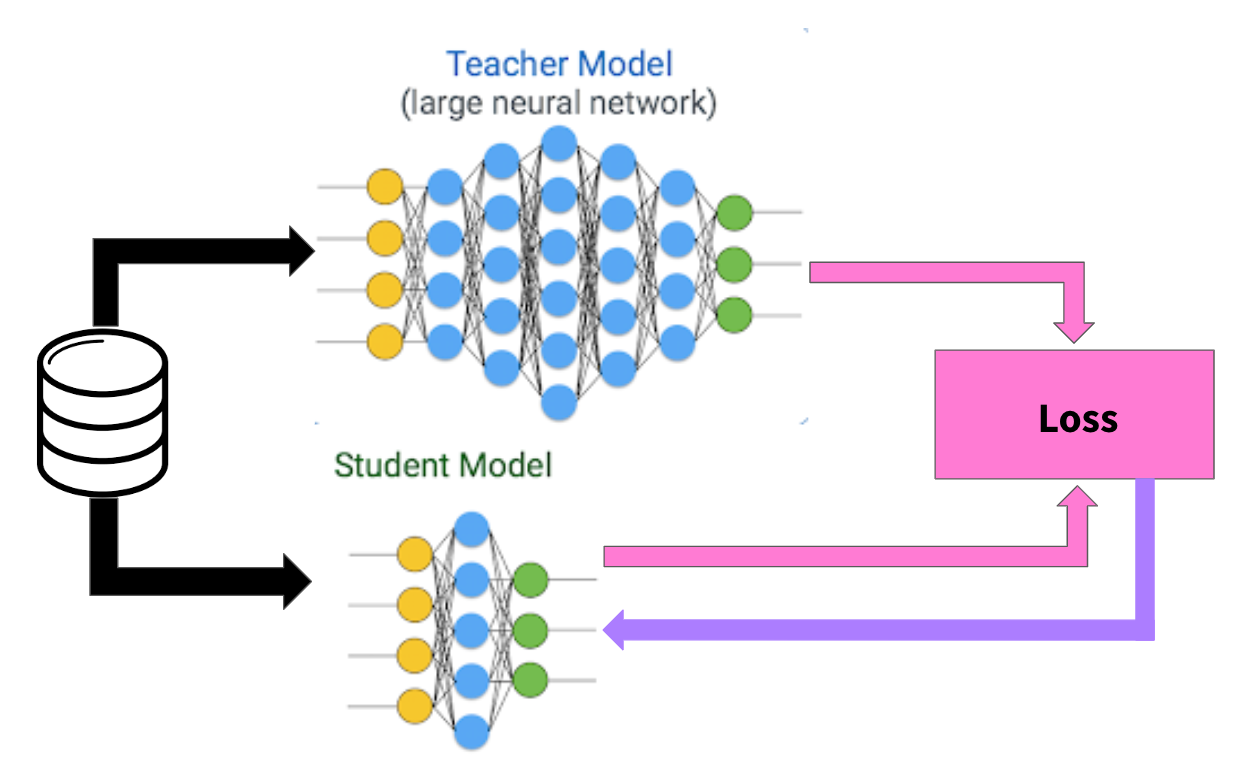
\includegraphics[width=\linewidth]{distillation.png}
%         \end{column}
%     \end{columns}
% \end{frame}

\begin{frame}{Conclusion}
    \myheading{Concerns}
    \begin{itemize}
        \item Despite the suitability of FPGAs for this task, could it be the case that GPUs are simply so good at ML tasks that the latency overhead wouldn't matter?
    \end{itemize}

    \myheading{Highlights}
    \begin{itemize}
        \item I've enjoyed looking into ML implementations at a lower level and I'm excited to begin swapping out some of my implementations with real FPGA hardware.
    \end{itemize}

    \begin{block}{Summary}
        Our goal is to achieve real-time HSI classification using a custom FPGA implementation. The real-time nature of this implementation would be highly useful for field work and real applications, but requires overcoming engineering challenges related to our hardware.
    \end{block}
\end{frame}


\begin{frame}{Acknowledgements}
    \begin{itemize}
        \item This material is based upon work supported by the National Science Foundation under Grant No. 2349091.
        \item I would like to acknowledge my PI Ross Snider for the direction and assistance he has provided on the project.
        \item I would also like to thank Nat Sweeney, Zackery Backman, and Dirk Kaiser for the work that they have done and continue to do on the project.
    \end{itemize}
\end{frame}


% I think I just need to add citations for the presentations I was shown (and tbh this is optional)
\begin{frame}[allowframebreaks]{References}
    \begingroup
    \tiny
    \setlength{\itemsep}{0pt}
    \setlength{\parsep}{0pt}
    \setlength{\parskip}{0pt}
    \nocite{*}
    % \setlength\bibitemsep{0.3ex}
    % \printbibliography[heading=none]
    \bibliographystyle{acm}
    \bibliography{reference.bib}
    \endgroup
\end{frame}

\begin{frame}
    \Huge{\centerline{\textbf{The End}}}
\end{frame}

\end{document}
